%%%%%%%%%%%%%%%%%%%%%%%%%%%%%%%%%%%%%%%%%%%%%%%%%%%%%%%%%%%%%%%%%%%%%%%
%      SEC. 1
%%%%%%%%%%%%%%%%%%%%%%%%%%%%%%%%%%%%%%%%%%%%%%%%%%%%%%%%%%%%%%%%%%%%%%%
\section{Introduction and structure of the thesis}

Passion and curiosity should always lie at the heart of the scientific practice, and that ought to be enough to define the value of a research effort~\cite{Weber1917,Shapin2015}. Time is the real arbiter of the significance of a piece of research, as many examples in the history of science show~\cite{Brush1967,Niss2008}\footnote{The Ising-Lenz model is one such example~\cite{Brush1967,Niss2008,Niss2004}. It was suggested by physicist Wilhelm Lenz to his doctoral student Ernst Ising to study phase transitions in ferromagnetic materials. Ising solved it analytically in 1D as part of his Ph.D. defense in 1925, but the solution for a 1D lattice did not show any phase transition. This apparent failure is thought to be the reason of Ising's decision to take a job outside academia. Almost 20 years later, Onsager solved the 2D version of the model and showed the possibility of phase transitions in the Ising-Lenz model. By the time Ising arrived in the USA in 1947, the Ising-Lenz model was already entering the canon of physics and, to his surprise, he was being asked if he was ``the Ising" of the ``Ising model".}.However, in these years of increasing mistrust towards scientific research and brewing doubts about the value of universities and research institutes~\cite{Biesta2002,Biesta2004,Santos2012}, it is worthwhile to try to place one's own work into the wider picture of one's own time. It is also a valuable exercise for the researcher, who sensibly progresses in the work by investigating one detail at a time, to spend a moment away from one's own graphs and equations and see their place in the wider perspective of the world outside the laboratory.\\
It is thus in this spirit that I propose to open the present work with a reflection on the challenges that the transportation industry faces at the closing of $21^{st}$ century's second decade. Against this background, in Chapter~1 \emph{thin-ply} laminates are introduced as a very promising material for innovative structural design and their main characteristics are discussed. The focus is then moved to the most renown quality of thin-ply laminates, i.e. their ability to delay and even suppress onset and propagation of transverse cracking, and to discuss the modeling issues that this new material poses. A link is established with the growth of fiber/matrix interface cracks or, as very often called in the rest of the thesis, debonds. The fiber/matrix interface crack is then discussed in detail, and previous analytical, computational and experimental studies available in the literature are reviewed. The modeling strategy adopted in this thesis is then presented and its implementation described. Finally, Chapter~3 provides a summary of the main results of this work, organized following the order of the publications reported in Part~II of the thesis. The first chapter is thus a journey of scales: we start from the challenges of an industrial sector, move to the structural requirements of its products, focus on a promising new material, and concentrate on understanding the mechanisms of damage initiation and propagation.

\section{Vision 2030: challenges of the next decade and beyond for the transportation industry}

The closing of the second decade of the $21^{st}$ century brings different challenges for the transportation industry, which will likely shape its development in the next decade and beyond. A brief review of the most relevant aspects is proposed here.

\begin{description}
\item[Climate action.] The issue of climate change is certainly one the ``hot" topic of today's public debate. A discussion of the merits of scientific understanding of climate change, public reception, media coverage and socio-political implications is out of the scope of the present work, but it is certainly one of the most relevant topic framing today's public discourse. Given that it is a high-divisive subject, no judgement on the validity of the claims of one side or the other is proposed here, as sufficient space can not be devoted to a thorough analysis of the problem. What is acknowledged here is the emergence of concerted efforts at the institutional level (companies, city administrations, regional governments, sovereign states) to rule into and provide control mechanisms to limit the emission of carbon dioxide, i.e. $CO_{2}$. The evidence of this shift in public policy is exemplified in Figure~\ref{chap1:fig:climatedealssignataries} and Figure~\ref{chap1:fig:greenfundpledges}.\\ Figure~\ref{chap1:fig:climatedealssignataries} reports the evolution over time of the number of signatories of three representative deals on climate action. The selected deals are: the Vienna Convention for the Protection of the Ozone Layer, first signed in 1985 and committing signatories to the reduction of chlorofluorocarbons; the United Nations Framework Convention on Climate Change (UNFCCC), initially agreed in 1992 with the aim of managing the increase in greenhouse emission in order to avoid dangerous interferences with the climate; the Kyoto Protocol, signed in 1997 as an extension of the UNFCCC and according to which adhering countries pledge to reduce greenhouse emissions to prevent climate change. Figure~\ref{chap1:fig:climatedealssignataries} shows how the majority of countries have ratified these deals over time, reaching an almost unanimous agreement on the need of coordinated action towards the issues of climate change.

\begin{figure}[!h]
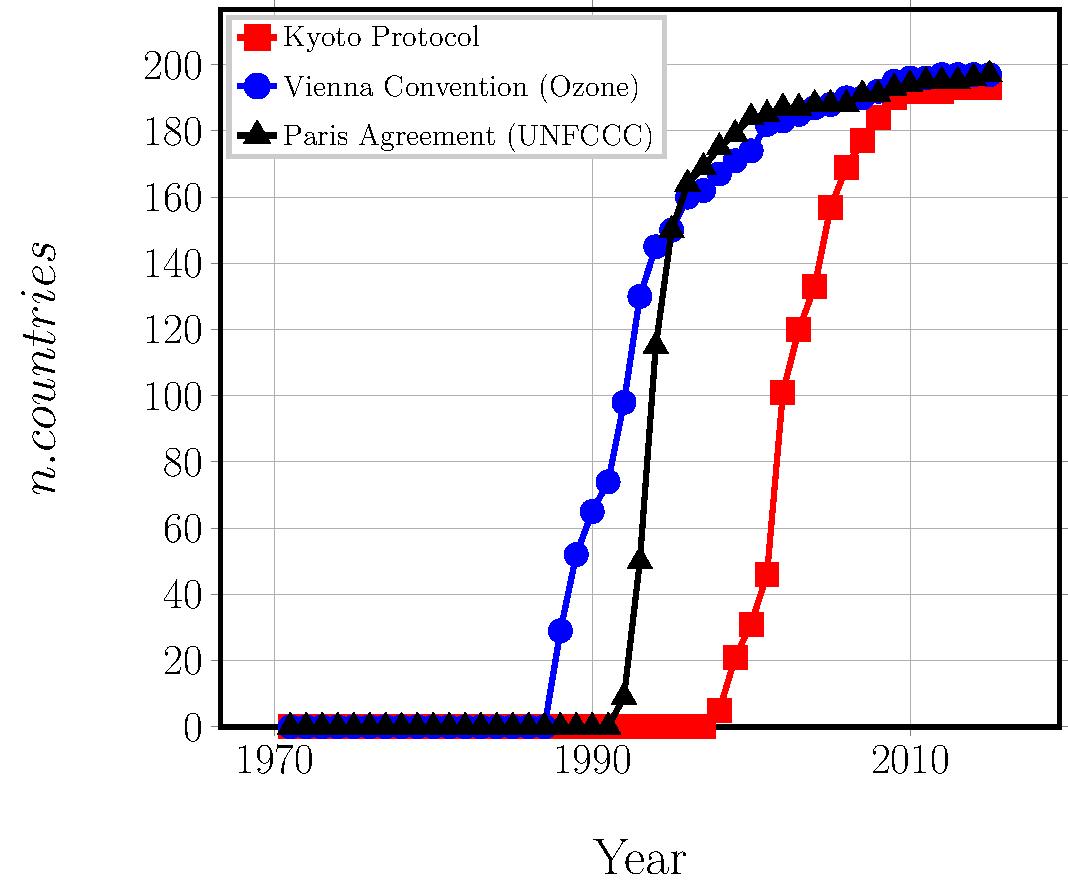
\includegraphics[width=0.9\textwidth]{pics/climate-deals-signataries.pdf}
\caption{Number of signing countries over time for selected deals on climate. Source: UNCTAD Development and Globalization: Facts and Figures (2016). United Nations Conference on Trade and Development. Available at \href{https://stats.unctad.org/Dgff2016/DGFF2016.pdf}{https://stats.unctad.org/Dgff2016/DGFF2016.pdf} (last access: September 26, 2019).}\label{chap1:fig:climatedealssignataries}
\end{figure}

Figure~\ref{chap1:fig:greenfundpledges} shows the 10 highest contributions to the Green Climate Fund, which aims to support projects in developing countries focusing on reduction of greenhouse gas emissions and climate adaptation. The commitment to this effort of industrialized countries is evident in Figure~\ref{chap1:fig:greenfundpledges}. It is thus apparent from Figure~\ref{chap1:fig:climatedealssignataries} and Figure~\ref{chap1:fig:greenfundpledges} that a shift in public attitude and policy towards the issues of climate change has been under way in the last decades. This shift in turn has been materialized in the form of international agreements on climate action, which have led to the introduction of novel regulations aimed at containing the emission of $CO_{2}$ and other pollutants into the atmosphere and biosphere at large.

\begin{figure}[!h]
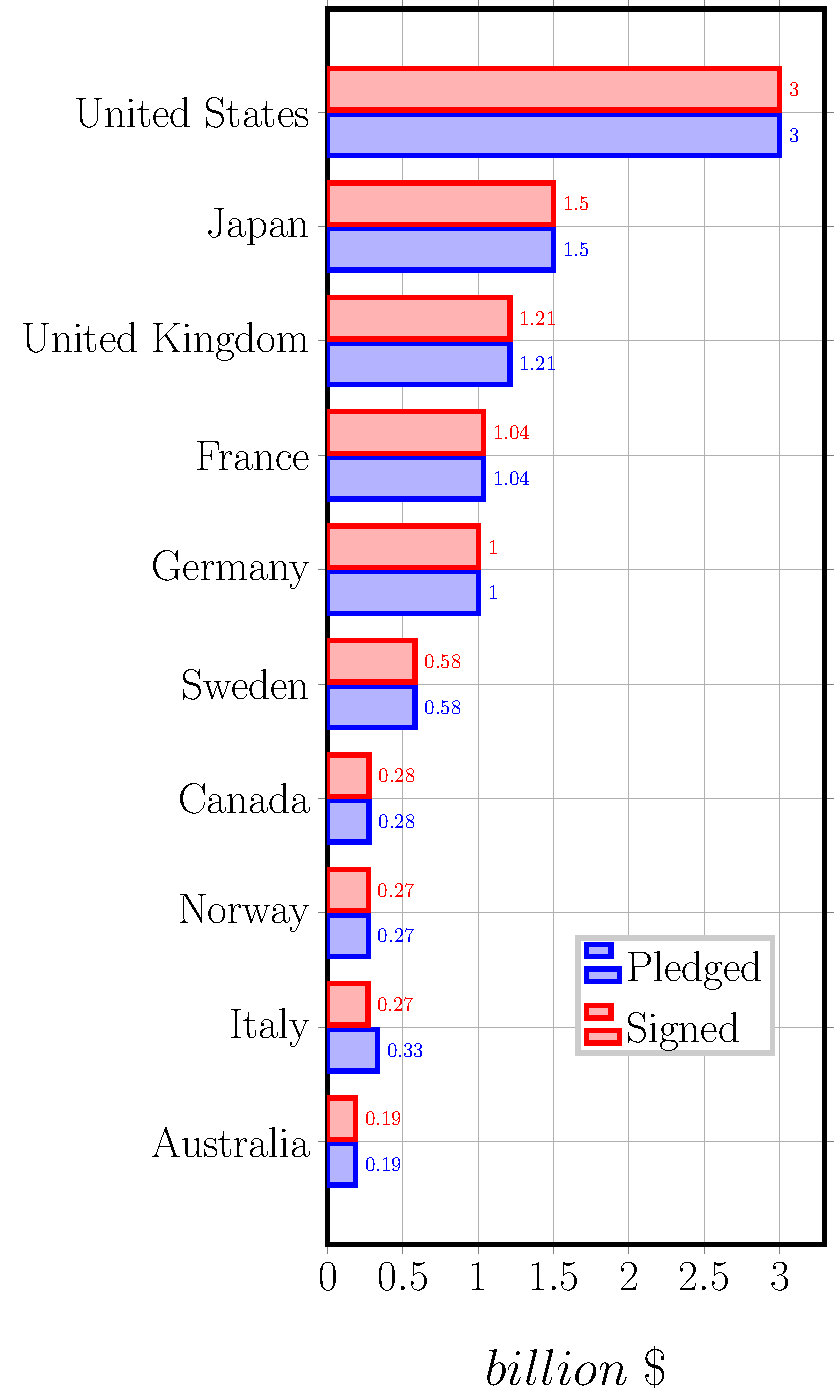
\includegraphics[height=0.75\textheight]{pics/green-fund-pledges.pdf}
\caption{Pledged and signed contributions to the Green Climate Fund of the 10 countries with the highest signed contributions. Source: Green Climate Fund, available at \href{https://www.greenclimate.fund/how-we-work/resource-mobilization}{https://www.greenclimate.fund/how-we-work/resource-mobilization} (last access: September 21, 2019).}\label{chap1:fig:greenfundpledges}
\end{figure}

It is interesting to understand the impact of this shift on the transport industry by looking at some representative data of its $CO_{2}$ emissions. In Figure~\ref{chap1:fig:co2transportshare} the share of total $CO_{2}$ emissions is reported for some selected countries. The first observation is that the role of the transport industry as a source of $CO_{2}$ has been increasing over the years. Today it accounts for around $30\%$ of total emissions in large mature economies such as the United States and the European Union, around $20\%$ of Japan's emissions and $10\%$ of China's.

\begin{figure}[!h]
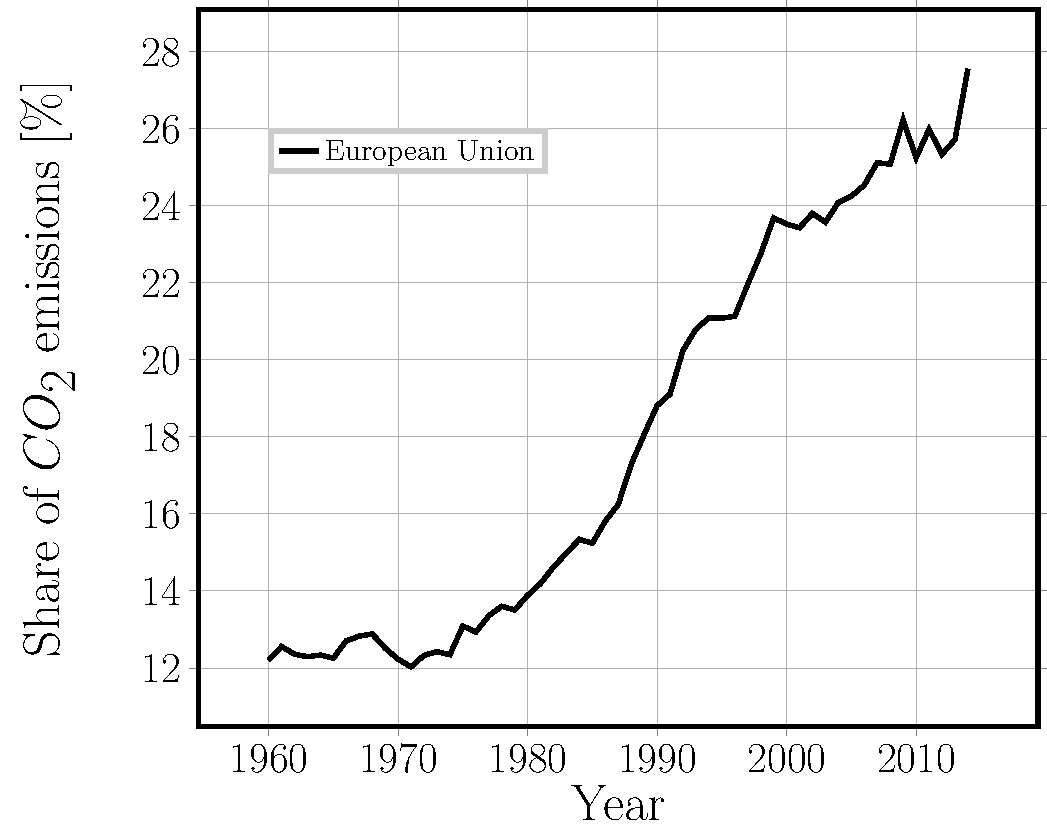
\includegraphics[width=0.9\textwidth]{pics/co2transportshare.pdf}
\caption{Share of total $CO_{2}$ emissions due to the transport sector over time for selected countries. Source: International Energy Agency (IEA) via The World Bank, available at \href{http://data.worldbank.org/data-catalog/world-development-indicators}{http://data.worldbank.org/data-catalog/world-development-indicators} (last access: September 21, 2019).}\label{chap1:fig:co2transportshare}
\end{figure}

A second perspective on the problem in provided in Figure~\ref{chap1:fig:co2transportabsolute}, where the evolution of $CO_{2}$ total emissions (in absolute terms) for selected world geographical entities is compared with that of international transport. Interestingly, the emissions of the latter has been comparable in the last 50 years to those of the African continent as a whole.

\begin{figure}[!h]
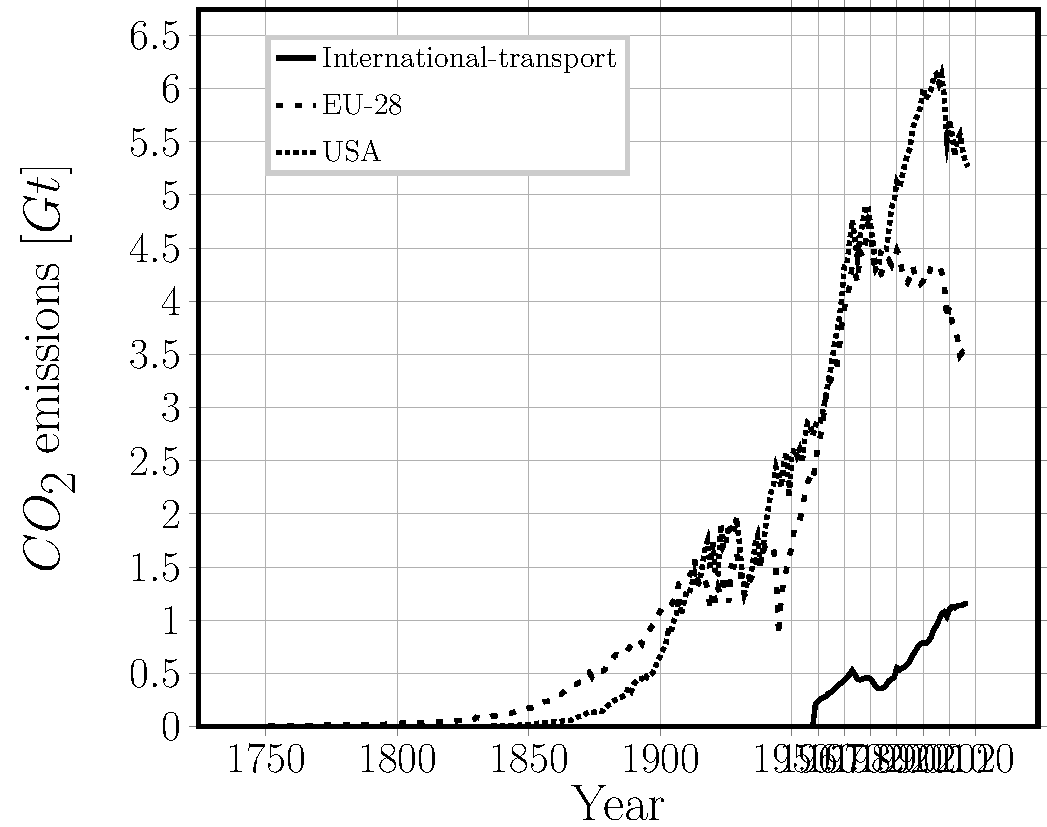
\includegraphics[width=0.9\textwidth]{pics/co2transportabsolute.pdf}
\caption{Total $CO_{2}$ emissions due to transport over time, compared with selected geographical entities. Source: The Global Carbon Project, available at \href{https://www.globalcarbonproject.org/}{https://www.globalcarbonproject.org/} (last access: September 21, 2019).}\label{chap1:fig:co2transportabsolute}
\end{figure}

It is thus clear from Figure~\ref{chap1:fig:co2transportshare} and Figure~\ref{chap1:fig:co2transportabsolute} that the transport sector plays a prominent role in the emission of $CO_{2}$ and other pollutants into the biosphere. It is, and will be, strongly affected by the emphasis on climate change that currently characterizes international public policy. Stricter standards on emissions are planned or expected in several parts of the world and the transport industry, currently one the biggest emitter, needs to innovate to adapt to this change.

\item[Increased competitiveness.] During the last couple of decades, the arrival of new players and the introduction of new business models have increased competitiveness in the transport sector and favored a downward pressure on prices. Several examples exist. In civil aviation, the diffusion of low-cost carriers such as Ryanair$^{TM}$, easyJet$^{TM}$ and Norwegian$^{TM}$, which offer very (and sometimes even extreme) low rates by drastically reducing the number of ancillary service comprised in the ticket price, which are then offered as pay-as-you-go additional services. The space sector has seen the arrival of a number of private actors which are developing or are already proposing on the market low-Earth launching technologies significantly cheaper than market incumbents. In the car industry, ride-sharing (such as BlaBlaCar$^{TM}$) and ride-hailing services (like Uber$^{TM}$ and Lyft$^{TM}$) are leading to a change in the importance of car ownership and, thus, in the role of car manufacturers.

\begin{figure}[!h]
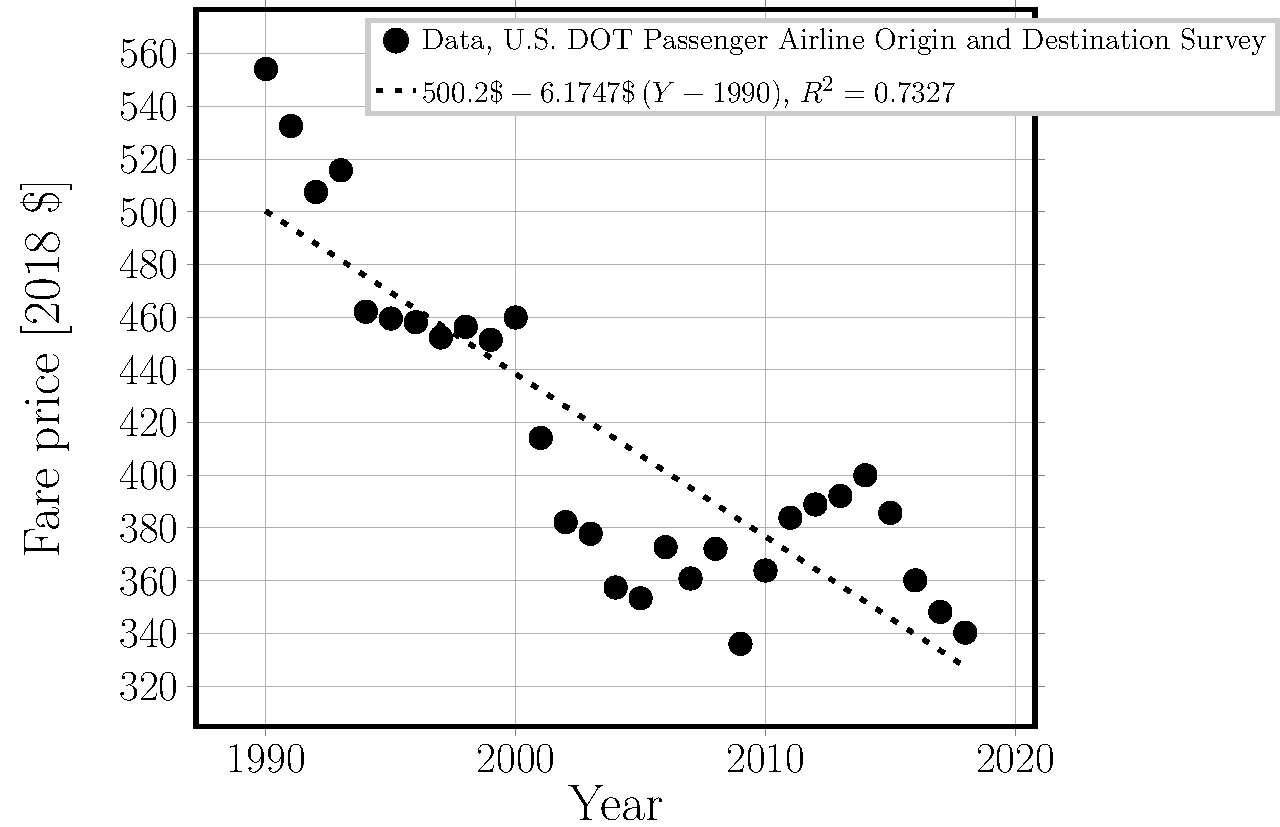
\includegraphics[width=0.9\textwidth]{pics/airlinefarecost.pdf}
\caption{Average airline fare in the United States over the years, prices in $2018\ \$$. Source: , available at \href{}{} (last access: , 2019).}\label{chap1:fig:airlinefarecost}
\end{figure}

Two representative examples of the reduction of prices over time in the transport industry are shown in Figure~\ref{chap1:fig:airlinefarecost} and in Figure~\ref{chap1:fig:spacetravelcost}. In Figure~\ref{chap1:fig:airlinefarecost}, the evolution of fare prices (expressed in 2018 US \$) over the past three decades in the United States is reported. A clear downward trend is observable and a linear regression of the data provides a negative slope with a $R^{2}$ coefficient of $0.7327$. Figure~\ref{chap1:fig:spacetravelcost} presents the unit cost (expressed in 2018 US \$) of payload for several different launch system with respect to time. Three systems are in particular highlighted: the Vanguard, the first one in history; the Space Shuttle, for introducing the concept of launch system reusability; the Falcon Heavy, for bringing to the market a privately managed reusable launcher system. Albeit with some scatter, it is possible to observe a downward trend of prices. A linear regression of the logarithm of price with respect to time provides an estimate of the year-on-year price decrease at around $3\%$, i.e. a $30\%$ every decade.

\begin{figure}[!h]
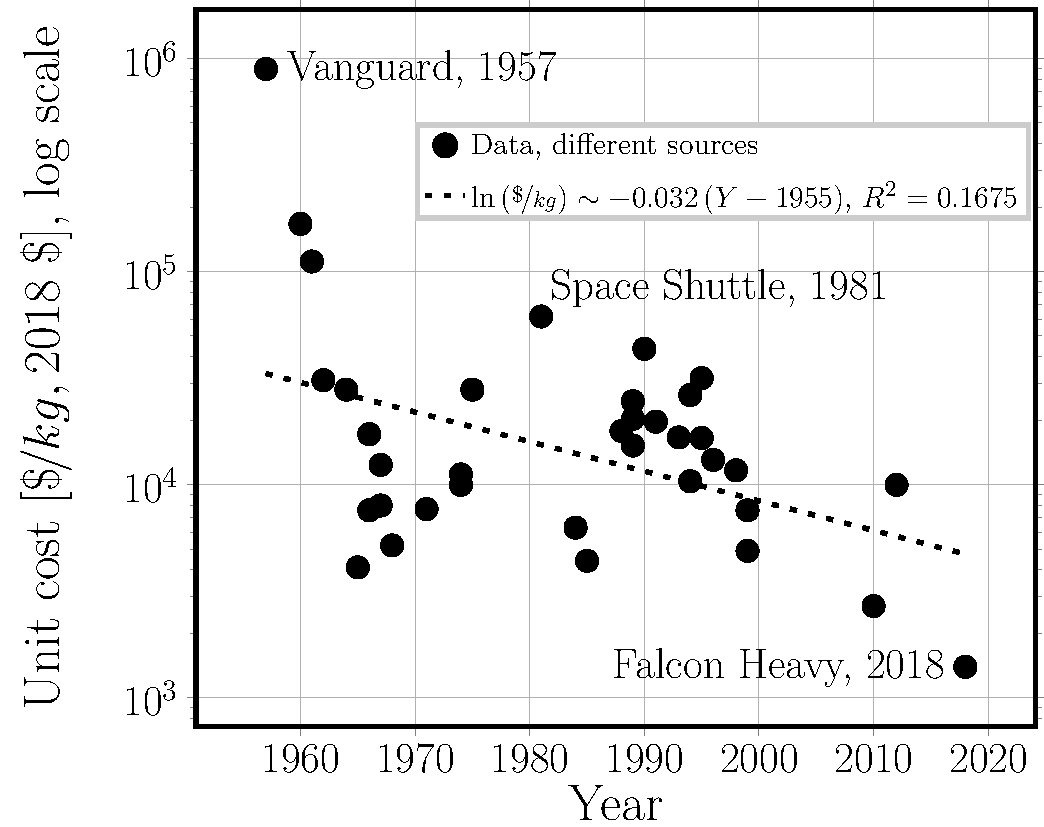
\includegraphics[width=0.9\textwidth]{pics/spacetravelcost.pdf}
\caption{Evolution of unit cost of payload for different launching over time, prices in $2018\ \$$. Source: , available at \href{}{} (last access: , 2019).}\label{chap1:fig:spacetravelcost}
\end{figure}

\item[Safety and crashworthiness.] Strict requirements on vehicles safety and crashworthiness are not a novelty of the 2010's, as legislation has been built over the years to create a system of control and verification to ensure that vehicles' structures are reliable under normal operating life as well as exceptional conditions. However, the recent crashes of the two Boeing 737 MAX 8 planes of Lion Air in Indonesia~\cite{aviationSafety2018} and of Ethiopian Airlines in Ethiopia~\cite{aviationSafety2019} have put the issue of safety and crashworthiness back into the spotlight, as the cause of the crashes was a technical glitch in the automatic guidance and control system. Thus, although the problem is one of software development and control system engineering, it calls for a revision of current practices of oversight and certification. For the structural designer, requirements of safety and crashworthiness translate into a thorough understanding of structural failure mechanisms, and thus of the evolution of damage in the materials employed.

\end{description}

These issues are framing the evolution of the transport industry over the next decade, particularly in technological terms. Their requirements are often incompatible and current solution represents often a trade-off between them. Renewed efforts are thus devoted to the development of materials that could satisfy at the same time the needs of sustainability, price reduction and structural safety.

\section{\textit{Thin-ply} laminates and the \textit{spread tow} technology}

A very promising material introduced into the market by the composite industry in recent times is the so-called \emph{thin-ply} laminate, result of a series of advancements in the \textit{spread tow technology}. Conventionally, fibers are produced as bundles or \textit{tows} comprising $12/24k$ filaments; tows are then stacked together and impregnated in order to produce prepreg plies. At the heart of the \textit{spread tow technology} lies the idea of opening or \textit{spreading} such tows to create thinner and wider tapes, to be then used in the production of unidirectional (UD) prepregs or woven fabrics, as schematically depicted in Figure~\ref{chap1:fig:spreadtowtech}.

\begin{figure}[!h]
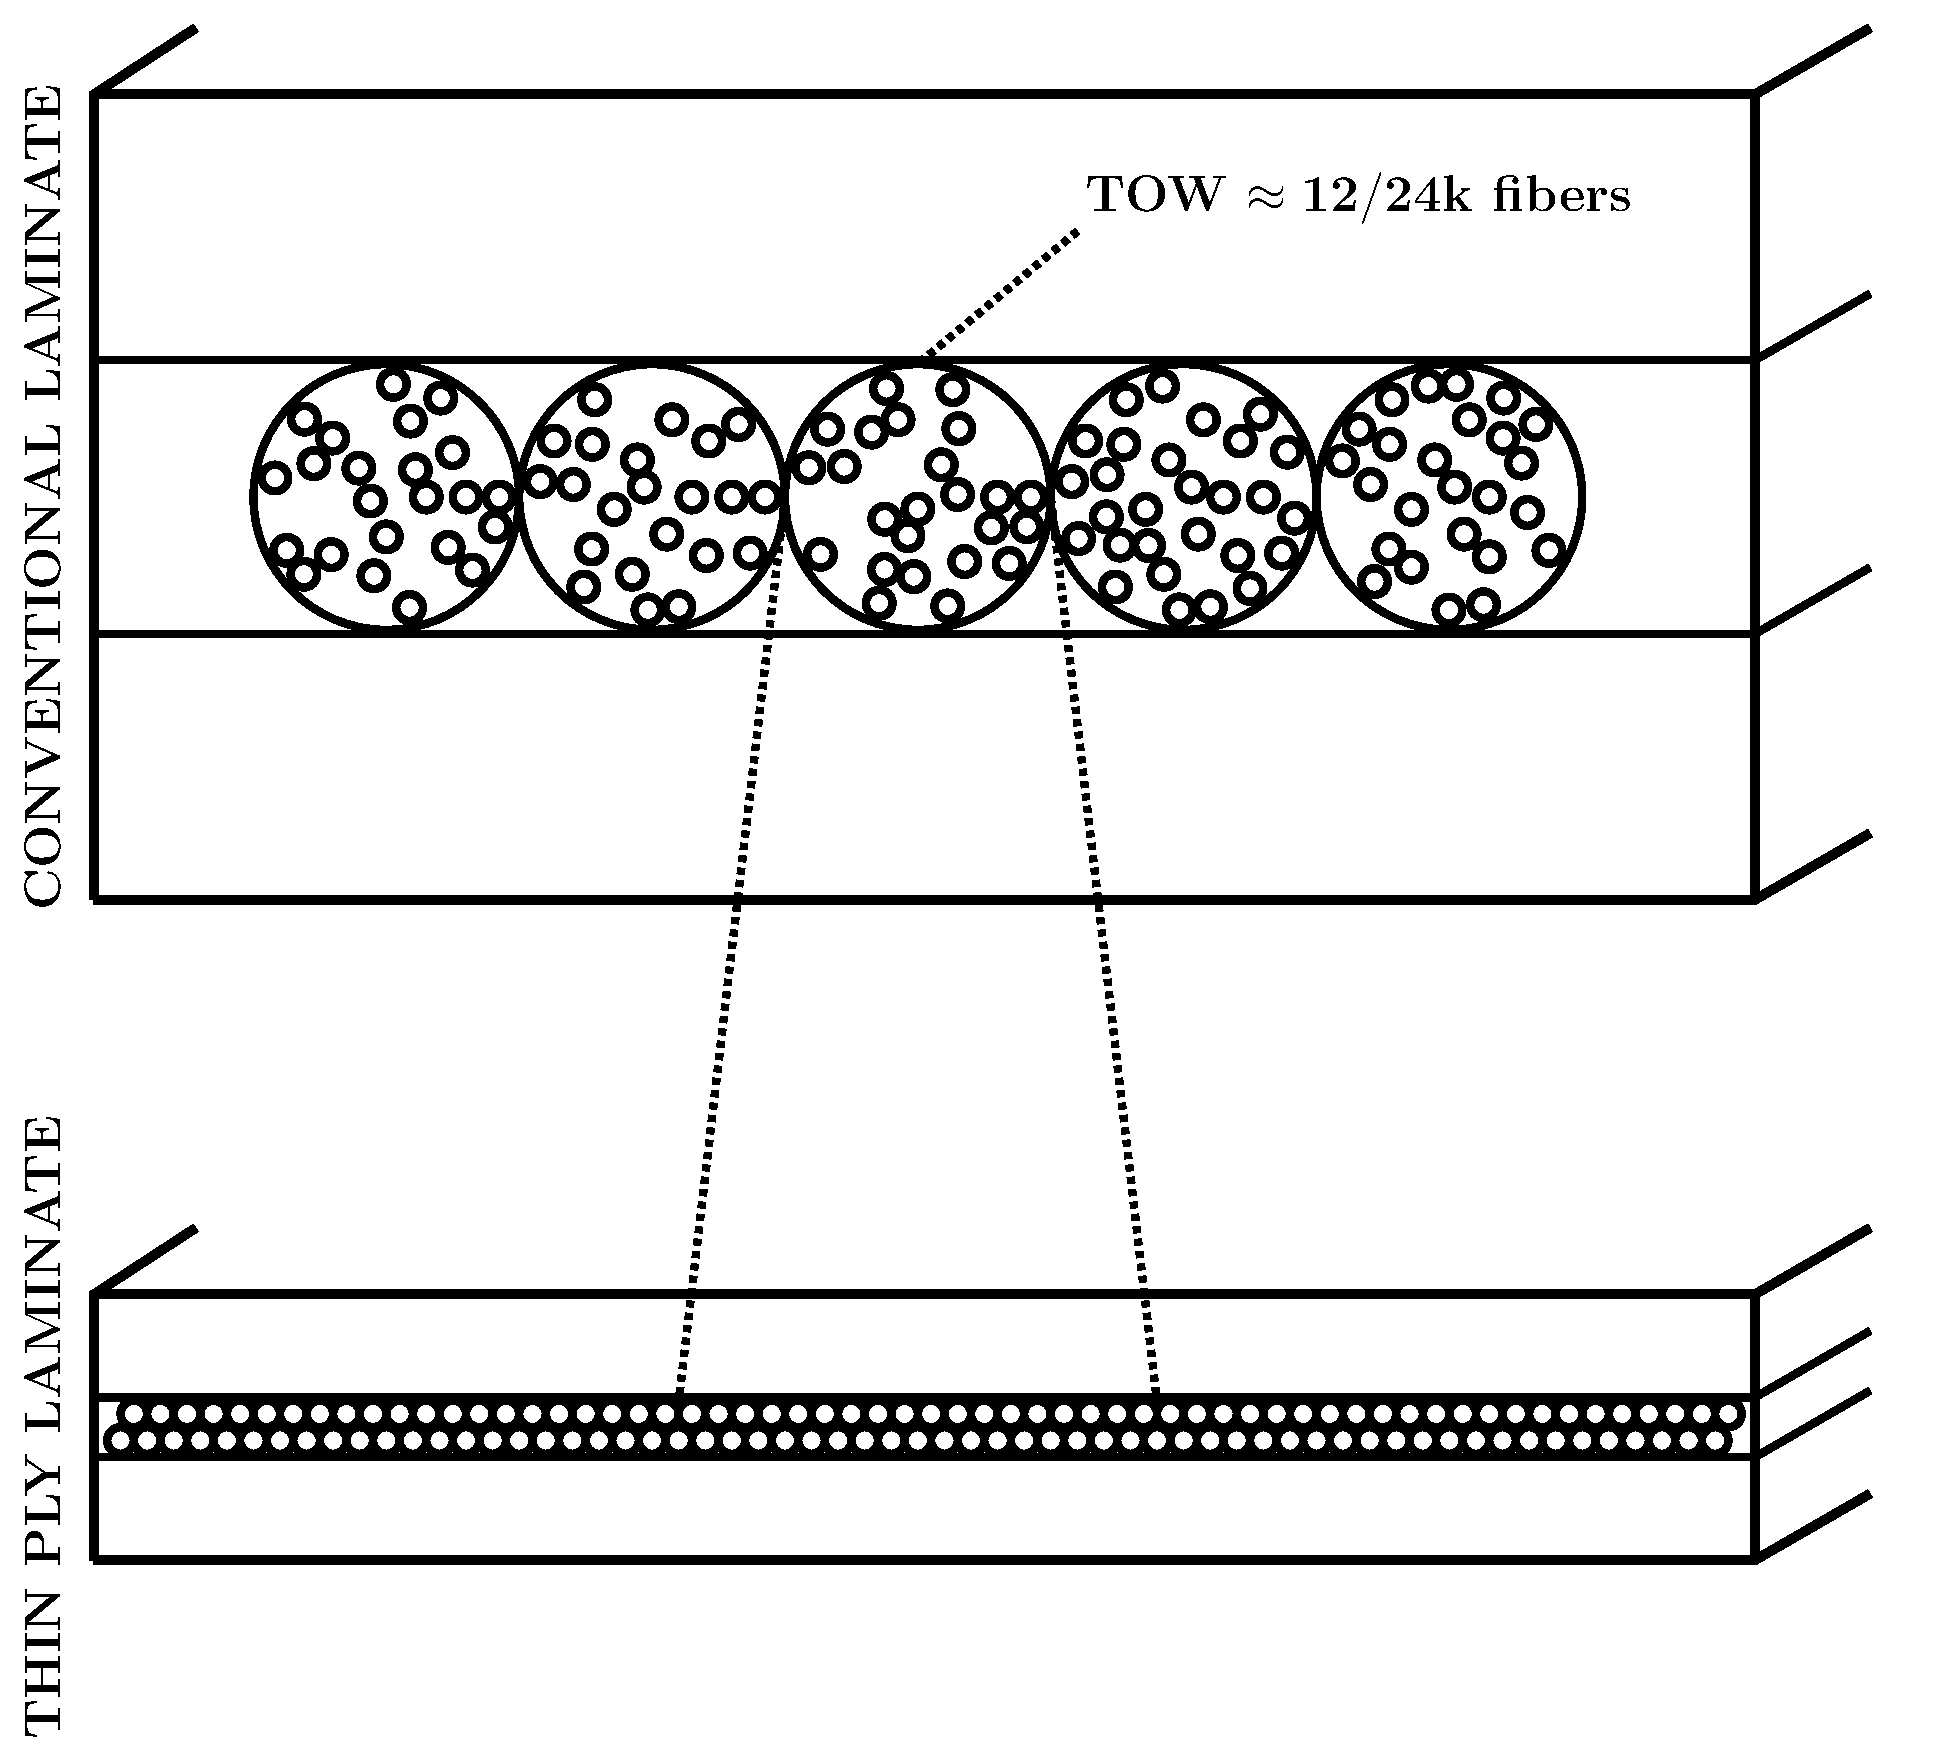
\includegraphics[width=0.75\textwidth]{pics/spread-tow-tech.pdf}
\caption{Schematic of the difference between laminates with conventional prepreg plies and \emph{thin-ply} laminates, issued from the \textit{spread tow technology}.}\label{chap1:fig:spreadtowtech}
\end{figure}

First attempts to turn the idea into practice date back to the 1970's~\cite{spreadtowpatent:1974}, when a Venturi injector opposite to the pulling direction of fibers was employed to split the tow. Other methodologies were then proposed, among others: acoustic vibrations in air generated by a speaker or similar apparatus below the tow~\cite{spreadtowpatent:1991}; mechanical separation by means of cylindrical rollers~\cite{spreadtowpatent:1992}; the use of expandable elastic bands (or tubes) mounted on a rotating drum~\cite{spreadtowpatent:2000}; electrostatic separation employing a corona discharge~\cite{spreadtowpatent:1993}. Nonetheless, they all suffered from a number of drawbacks: among the most critical, widespread breakages of fibers and deterioration of fiber surface properties, in particular wettability. A breakthrough arrived at the end of the 1990's, with the publication in 1997 of a contribution to the $42^{nd}$ SAMPE USA conference detailing a new spreading technique~\cite{Intro:KawabeTomodaMatsuo:1997} developed at the Industrial Technology Center in Japan's Fukui Prefecture. The so-called ``Fukui" technique (from the name of the Japanese prefecture), further improved in subsequent years~\cite{spreadtowpatent:2003,Intro:Kawabe:2008,Intro:SasayamaTomoda:2009}, is based on the combined use of focused air jets and a vacuum pump perpendicular to the pulling direction of fibers. Thanks to its capacity to avoid fiber breakage and fiber surface property loss, the technology has been applied on industrial scale to produce high-quality extremely thin fiber-reinforced prepreg plies. Only a few manufacturers exist today that produce thin-ply laminates, among them North Thin Ply Technology (NTPT)~\cite{ntpt} in Switzerland (founded in 2001), Oxeon~\cite{oxeon} in Sweden (founded in 2003), Chomarat~\cite{chomarat} in France, Sakai Ovex~\cite{sakai} in Japan. The technology is now reaching a mature stage and proposals have been made to use thin-ply laminates in primary load-carrying structural in safety critical applications such as Low-Earth Orbit (LEO) satellites~\cite{Moon2011}, airplane wings~\cite{Kim2017}, pressure vessels for cryogenic fuels~\cite{McCarville2018}, re-usable space launchers~\cite{Kopp2017}.\\
Probably the first assessment of the mechanical performance of thin-ply laminates was published by the developers of the \emph{spread tow} technology themselves in 2004 in the Journal of the Japan Society for Composite Materials~\cite{sasayamaJSCM2004}. They studied the effect of ply thickness on first-ply failure in quasi-isotropic carbon fiber laminates under static tensile loading and observed an increase of the value of the stress at first ply failure.  Soon after, K. Yamaguchi and H. T. Hahn~\cite{Yamaguchi2005} reported that, in cross-ply laminates subjected to static tensile loading, no transverse crack and no delamination was observed in the thin-ply specimen. According to the authors, fatigue behavior was also improved in thin-ply laminates: the rate of growth of micro-cracks density was slowed and no transverse-crack induced delamination appeared even after $10^{6}$ cycles. The same year (2005), two contributions~\cite{TsaiICCM2005,Tsai2005} by S. Tsai and collaborators confirmed these observations. They tested cross-ply and quasi-isotropic laminates in simple static tension, static open hole tension and fatigue, and observed the suppression of micro-cracking and transverse-cracking induced delaminations. A number of experimental studies on thin-ply laminates then followed, following the increasing interest from industry and responding to the need of the latter to characterize and standardize the properties of this new type of composite material. A comprehensive mechanical characterization of carbon fiber thin-ply laminates is described in~\cite{Sihn2007}. Here the authors compare the results of different tests between two different types of quasi-isotropic laminates, both made with the same number of ply and with the same \emph{spread-tow} but with different effective thicknesses of the layers: the first type, namely the ``thick" laminate, has layers made up by 5 plies for a thickness of $200\ \mu m$; the second, namely the ``thin" laminate, has layers made up by only 1 ply for a thickness of $40\ \mu m$. In the case of unnotched tension, the ultimate strength of the ``thin" laminate was found to be $10\%$ higher than that of the ``thick" laminate and no transverse crack was observed in the ``thin" laminate. Similarly, no micro-damage was detected in the ``thin" laminate in the case of unnotched tension-tension cyclic fatigue loading. The same observation was made in open-hole specimens under static tension and tension-tension fatigue loading, where practically no damage was observed in the ``thin" laminate. However, the final static failure of the ``thin" laminate occurred at a value roughly $10\%$ lower than that of the ``thick" laminate. In-depth ultrasonic scans of plates subjected to impact showed roughly equal delaminated areas between the two types of laminates, but Compression After Impact (CAI) tests seemed to point to a delay in the onset of buckling instability in the ``thin" laminate. However the analysis was not conclusive regarding the impact behavior of thin-ply laminates. A subsequent work~\cite{Yokozeki2008} addressed in more detail this point and focused on the experimental assessment of the compressive and impact behavior of thin-ply laminates. In particular, quasi-isotropic laminates made from standard and thin-ply prepregs made of the same carbon fiber/toughened epoxy system were subjected to static tensile tests, tension-tension cyclic fatigue loading, Non-Hole Compression (NHC), Open Hole Compression (OHC) and CAI tests. The results from static and fatigue tension confirmed the observations of~\cite{Sihn2007}. NHC and OHC tests showed an increase of respectively $16\%$ and $9\%$ of the final failure stress in thin-ply laminates with respect to conventional ones. C-scans after impact and CAI confirmed the results proposed in~\cite{Sihn2007}: delamination areas of similar size but CAI strength $8\%$ higher in thin-ply laminates. The same authors later investigated the response of thin-ply laminates to out-of-plane transverse loads~\cite{Yokozeki2010}, comparing quasi-isotropic laminates made of standard and thin-ply prepreg employing the same carbon fiber/toughened epoxy material system subjected to transverse indentation. They analyzed the evolution of damage through X-ray inspection and reported significantly different damage growth behaviors between thin-ply and standard laminates. Saito and colleagues~\cite{Saito2012} conducted \emph{in-situ} edge observations of transverse crack onset and propagation in the central $90^{\circ}$ layer on thin-ply carbon fiber laminates under tensile loading. The laminates had different thicknesses, controlled by the number of thin-ply prepreg sheets used to manufacture the $90^{\circ}$ layer. The $0^{\circ}$ layer had always the same thickness and was made of a conventional carbon fiber prepreg. They reported that, by decreasing the thickness of $90^{\circ}$ layer, the occurrence of transverse cracks was delayed to higher levels of the applied strain and even, in the thinnest case (only one prepreg ply), suppressed. Recently, extensive experimental assessments of thin-ply laminates were conducted in~\cite{Amacher2014} and~\cite{Cugnoni2018}, with the aim of characterizing the effect of ply thickness, fibre, matrix and interlayer properties. Their results confirmed the previous observations on the delay and suppression of transverse cracking in thinner plies.\\
Looking at the different experimental investigations on thin-ply laminates, it seems apparent that there exists a point of agreement between all them. And it is that the main advantage of thin-ply laminates is their capability, increasing with decreasing layer thickness, to delay to higher levels of the applied strain, and for very thin layers even suppress, the appearance of transverse cracks and transverse-cracking induced delaminations. In turn it implies that thin-ply laminates undergo a path of damage evolution different from that observed in conventional laminates. Given that subcritical damage, like transverse cracks and transverse-cracking induced delaminations, appears later, or even not at all, in the loading process, the marked degradation of elastic properties observed in conventional laminates is not present in thin-ply ones. In laminates with very thin plies, where subcritical damage is suppressed, the final laminate failure has been recorded to occur practically at fiber failure strain level~\cite{Cugnoni2018}. This means that, on one side, thin-ply laminates can sustain much higher loads than the conventional counterpart without degradation of their mechanical properties, by using the same fiber and matrix materials and the same layups and by only changing the thickness of the plies. However, on the other hand, final laminate failure occurs more abruptly and in a very brittle manner, which makes the use of thin-ply laminates in structural applications more critical.

%\section{Onset and propagation of transverse cracking and the \emph{ply-thickness effect}}
\section{Onset and propagation of transverse cracking at the microscale: experimental observations and computational modeling}

The characteristic of thin-ply laminates to delay, and even suppress, the occurrence of transverse cracking is not actually a peculiarity of this material, but the result of a phenomenon, called \emph{ply-thickness effect} or also \emph{in-situ effect}, that has been observed much earlier in conventional laminates. When fiber reinforced polymer composites started to be used in primary structures in aeronautical applications during the 1960's, a comprehensive literature on failure mechanisms and damage accumulation processes in laminates was lacking~\cite{Hofer1967}. Researcher focused on the observation and quantification of failure mechanisms in glass fiber reinforced polymers~\cite{Hofer1967,Howe1972,Owen1972}, and later on in carbon fiber reinforced polymers. Working on glass fiber/epoxy cross-ply laminates subjected to tensile loading, Bailey and co-workers first observed the occurrence of transverse cracks~\cite{Garrett1977} (see Figure~\ref{intro:fig:transversecracks} for an example of transverse cracking in a glass fiber/epoxy specimen) at strain levels much lower than the matrix failure strain. They noticed that cracks run parallel to the reinforcement in the ply and were, on average, spaced evenly along the specimen, as exemplified in Figure~\ref{intro:fig:transversecracks}. They further observed that~\cite{Garrett1977,Parvizi1978a} the spacing between cracks decreased with decreasing $90^{\circ}$ layer thickness. Analysis of the stress-strain response in~\cite{Parvizi1978a} revealed the occurrence of a decrease in the elastic modulus in the absence of transverse cracks but associated with the appearance of a whitening effect. They provided the first account of the \emph{ply-thickness effect} in a subsequent work~\cite{Parvizi1978b}, where they reported, for glass fiber/epoxy cross-ply specimens, an increase in the value of the applied strain at which the first transverse crack spanning the whole specimen width was recorded. They referred to this value of the strain as $\varepsilon_{tu}$ and distinguished it from $\varepsilon_{ti}$, the value of the applied strain at which the first edge crack (not tunnelling through the width of the specimen) appeared. They also noticed that, for larger values of the $90^{\circ}$ layer thickness, values of $\varepsilon_{tu}$ and $\varepsilon_{ti}$ were close, as crack propagation through the thickness and through the width occurred almost instantaneously; for thinner $90^{\circ}$ layers, $\varepsilon_{tu}$ increased faster than $\varepsilon_{ti}$ as through-the-width tunnelling was much slower than through-the thickness propagation. At very low thicknesses, around $\sim100\ \mu m$, of the $90^{\circ}$ inner layer, transverse cracking was suppressed. The whitening effect first observed in~\cite{Parvizi1978a} was determined in~\cite{Bailey1979,Bailey1981} to be due to the appearance of fiber/matrix interface cracks (or debonds, shown in a glass fiber/epoxy specimen in Figure~\ref{intro:fig:debonding}). Fiber/matrix debonding was identified as the microscopic mechanism responsible for onset and propagation of transverse cracks~\cite{Bailey1979}.

\begin{figure}[!h]
\centering
    \begin{subfigure}[b]{0.3\textwidth}
    \centering
        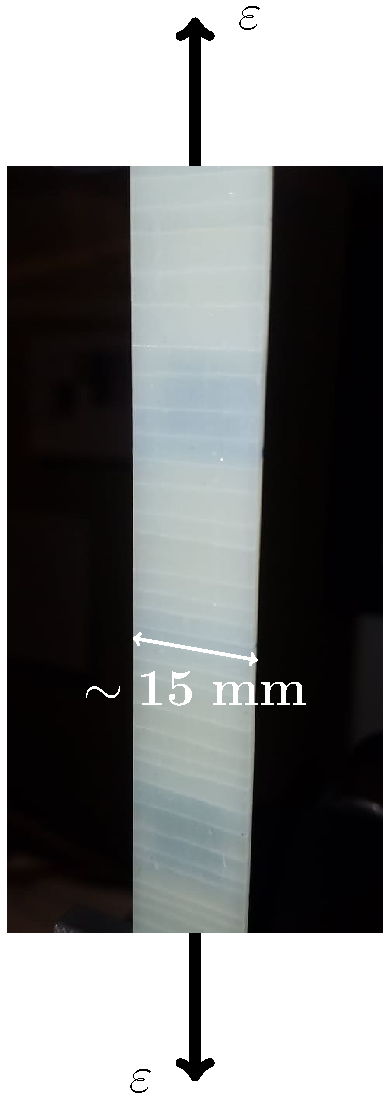
\includegraphics[height=0.75\textheight]{pics/transversecracks-macro.pdf}
       \caption{Front view, naked eye, $\left[0,90_{2}\right]_{S}$. The horizontal white lines are transverse cracks.}\label{intro:fig:transversecracks-a}
    \end{subfigure}
    \hfill
    \begin{subfigure}[b]{0.3\textwidth}
    \centering
        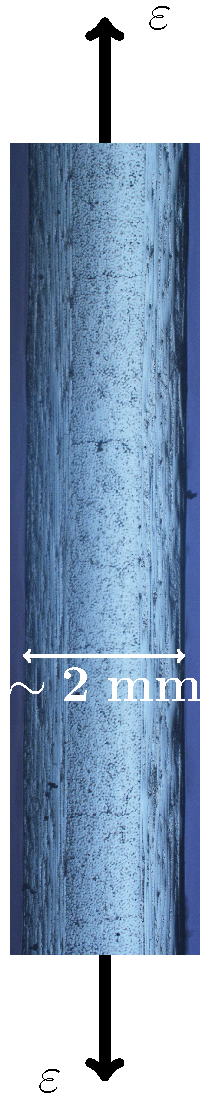
\includegraphics[height=0.75\textheight]{pics/transversecracks-meso.pdf}
       \caption{Edge view, optical microscope, $\left[0,90\right]_{S}$. The horizontal black lines in the central $90^{\circ}$ layer are transverse cracks.}\label{intro:fig:transversecracks-b}
    \end{subfigure}

\caption{Transverse cracking in glass fiber/epoxy cross-ply conventional laminates. Pictures taken by the author.}\label{intro:fig:transversecracks}
\end{figure}

Onset of debonding at the fiber/matrix interface was addressed by Asp and colleagues, who investigated the behavior epoxy under a tri-axial stress state as the one occurring in the inter-fiber regions~\cite{Asp1995}. They reported that, under such conditions, epoxy fails at very low strains ($\sim0.5\%-0.8\%$)~\cite{Asp1995} and in a brittle manner~\cite{Asp1996} through a cavitation-like failure mechanism taking place at, or extremely close to, the fiber/matrix interface. Debond growth was studied in two glass fiber/epoxy systems with in-situ optical microscopy on a single-fiber specimen under tension transverse to the fiber direction in~\cite{Zhang1997}. They observed debond growth along the fiber arc direction until a critical size, after which unstable growth in the fiber longitudinal direction occurred at approximately constant angular size. Recently, Scanning Electron Microscopy (SEM) and synchrotron-based 3D X-ray microtomography were applied to in-situ observations of fiber/matrix debonding in a glass fiber/epoxy single-fiber specimen under tension~\cite{Intro:Martyniuk2013}. The three dimensional quantitative assessment of debonding confirmed the previous observations presented in~\cite{Zhang1997}. The authors, in fact, reported debond initiation to occur at the specimen edge and at the same time at $0^{\circ}$ and at $180^{\circ}$ with respect to the loading direction. The initial size of debonds was measured and found to be $\sim18^{\circ}$. Then, the two debonds propagated symmetrically along the arc direction of the fiber until a critical size of $140^{\circ}$ (or $\Delta\theta=70^{\circ}$ following the nomenclature used in the rest of thesis) was reached. Finally, unstable propagation along the length of the fiber occurred, reaching conditions of self-similar steady-state growth at constant debond angular size of $48^{\circ}$ ($\Delta\theta=24^{\circ}$ after a small transition distance from the edge of the specimen.

\begin{figure}[!h]
\centering
        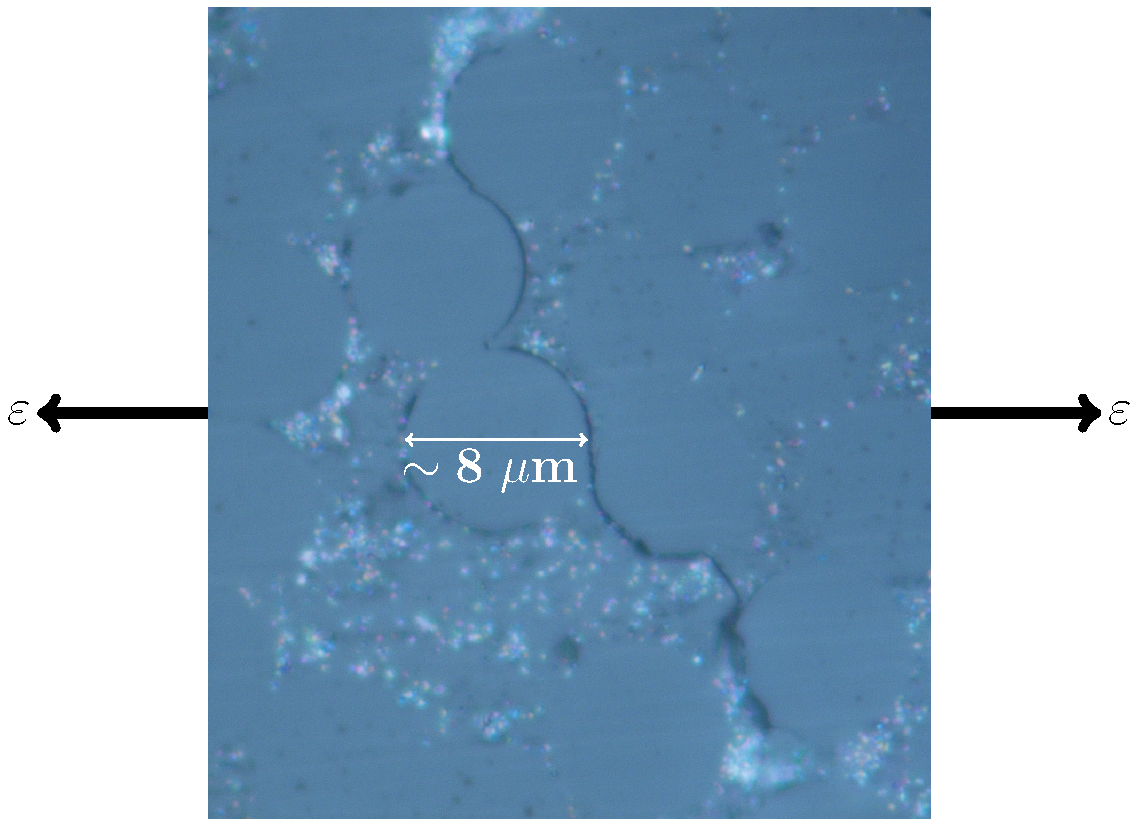
\includegraphics[width=0.9\textwidth]{pics/transversecracks-micro.pdf}
       \caption{Edge view, optical microscope, $\left[0,90\right]_{S}$.}
\caption{Debonding in glass fiber/epoxy cross-ply conventional laminates. The arc-shaped black lines are debonds at the fiber/matrix interface. Picture taken by the author.}\label{intro:fig:debonding}
\end{figure}

By taking an holistic view on the observations reported in~\cite{Garrett1977,Parvizi1978a,Parvizi1978b,Bailey1979,Bailey1981,Zhang1997,Intro:Martyniuk2013}, it is possible to propose a model of initiation and propagation of transverse cracking at the microscale in fiber-reinforced composites organized in several steps:

\begin{enumerate}
\item failure at the fiber/matrix interface occurs on a certain number of isolated fibers, i.e. not adjacent to another damage fiber, and an initial debond is formed (Figure~\ref{intro:fig:schematic-transversecracks-a});
\item stress re-distribution causes other interfaces to fail in the neighborhood, until a contiguous group of partially debonded fibers is present (Figure~\ref{intro:fig:schematic-transversecracks-b});
\item debond growth occurs along the arc direction until a critical size is reached, then the crack kinks out of the interface (Figure~\ref{intro:fig:schematic-transversecracks-a});
\item coalescence of debonds occurs and a through-the-thickness crack is formed (Figure~\ref{intro:fig:schematic-transversecracks-a});
\item the through-the-thickness crack tunnels through the width creating a transverse crack (Figure~\ref{intro:fig:transversecracks}).
\end{enumerate}

The model is certainly idealized, for example the distinction between step 2 and step 3 might be considered arbitrary. However, it provides a clear mental picture and a working model to categorize the analysis of this complex phenomenon.

\begin{figure}[!h]
\centering
    \begin{subfigure}[b]{0.45\textwidth}
        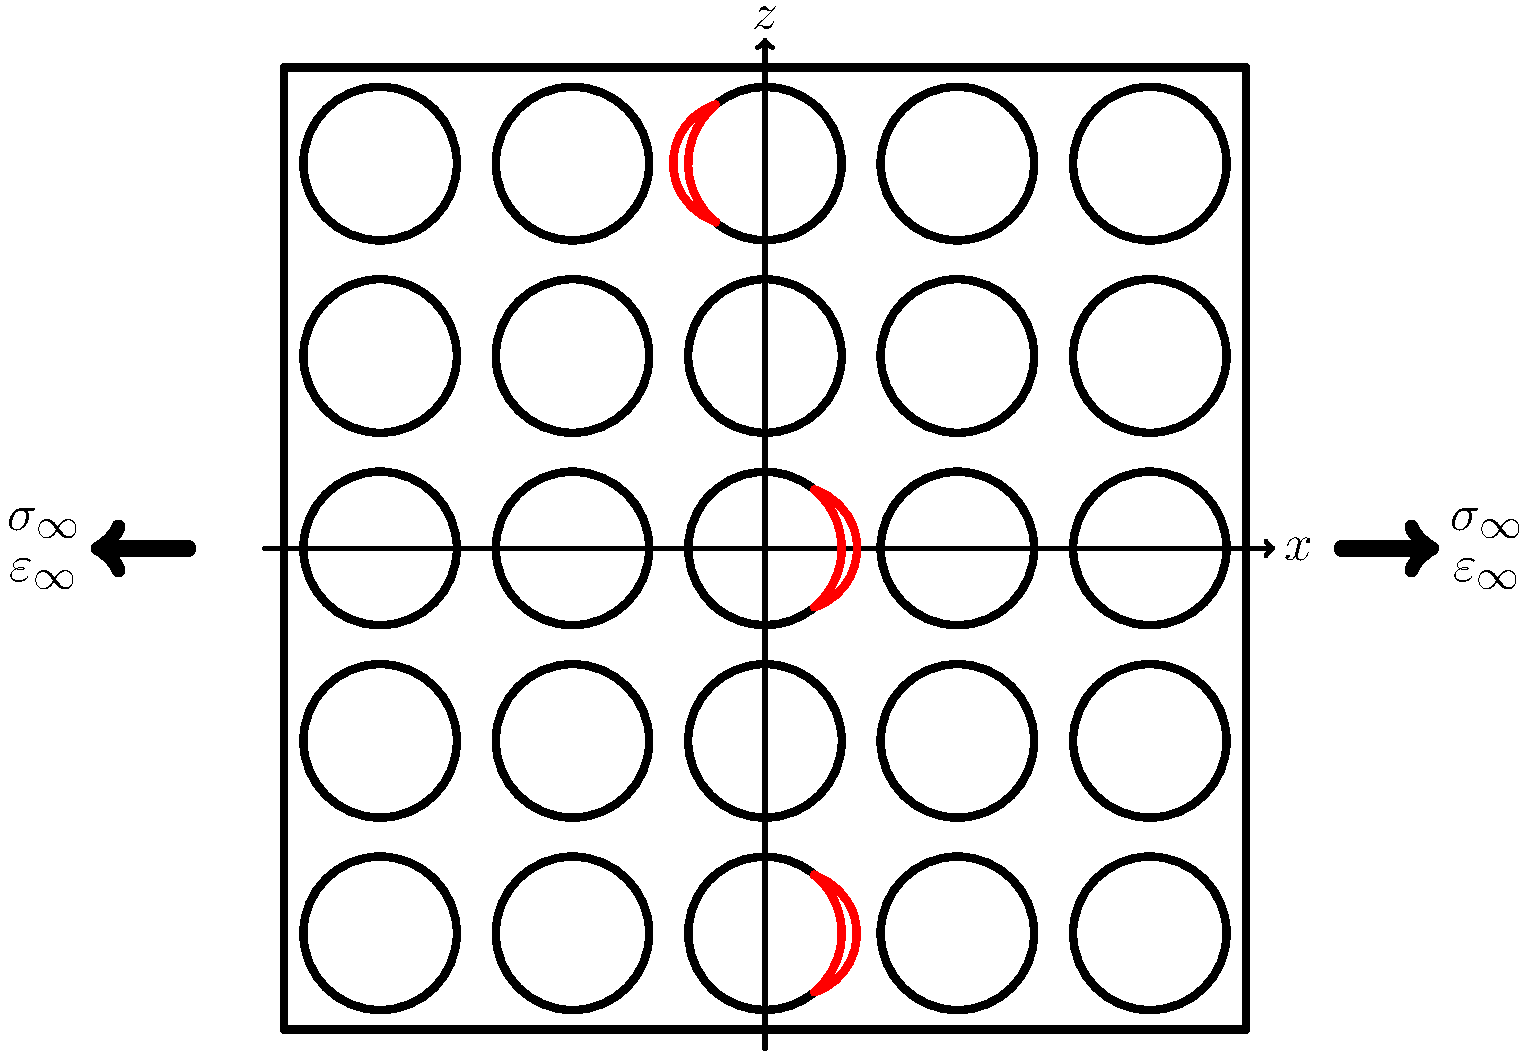
\includegraphics[width=\textwidth]{pics/stage1-isolateddebonds.pdf}
       \caption{Isolated debonds.}\label{intro:fig:schematic-transversecracks-a}
    \end{subfigure}
    ~
    \begin{subfigure}[b]{0.45\textwidth}
        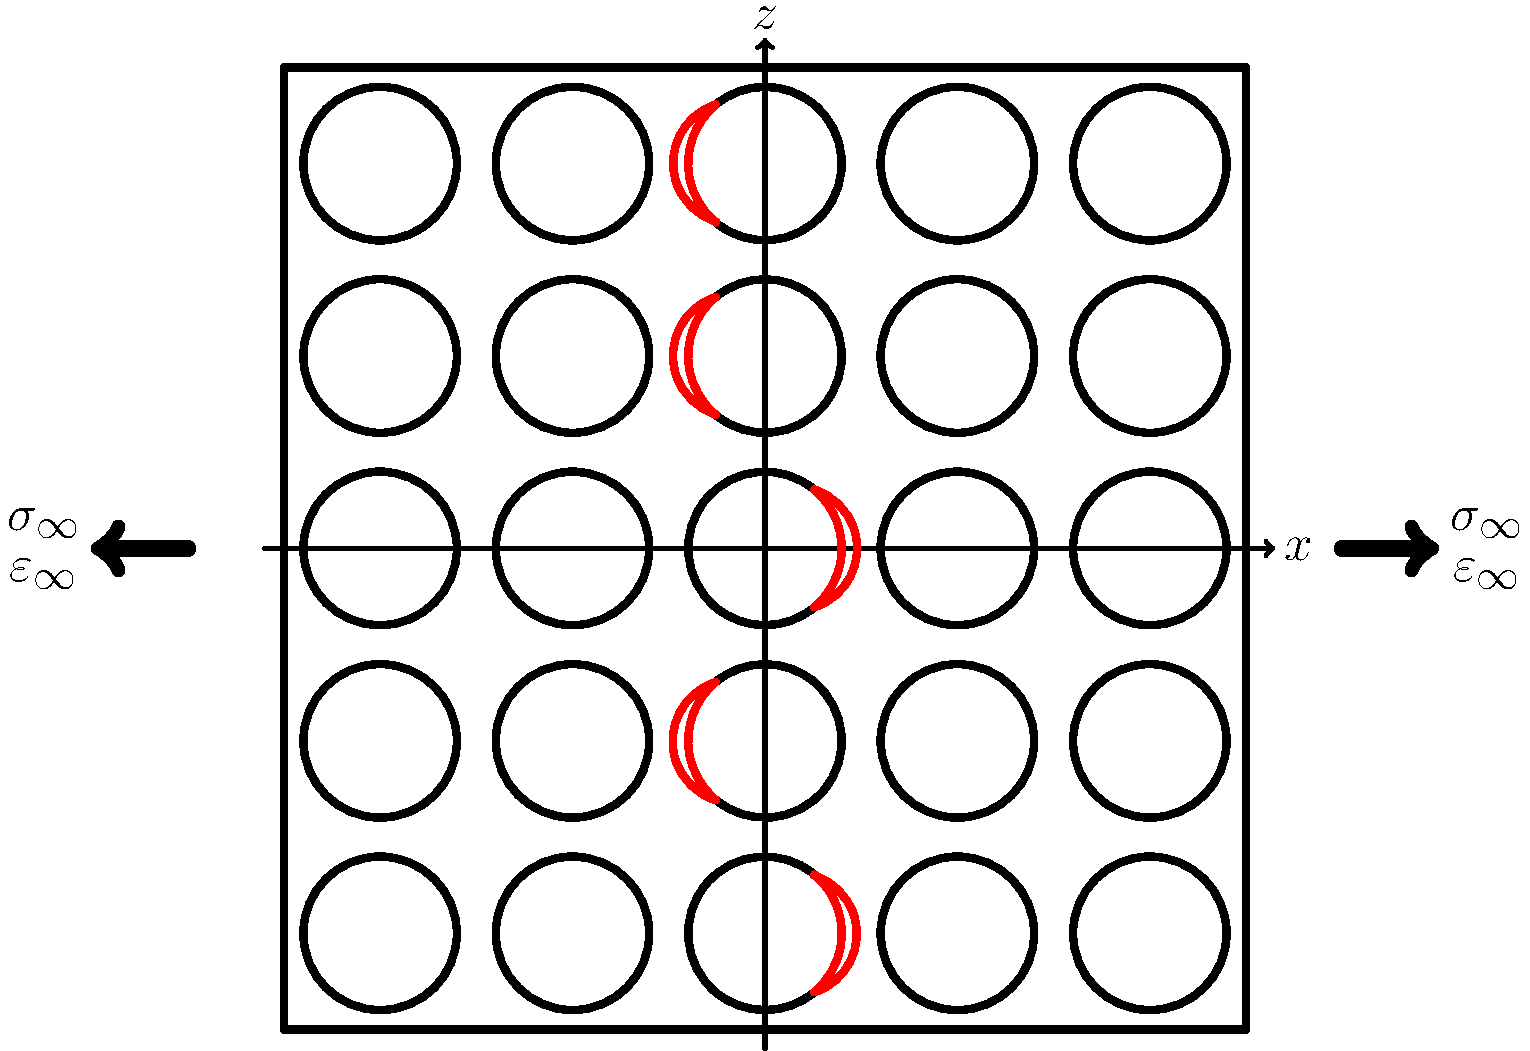
\includegraphics[width=\textwidth]{pics/stage2-critdebonds.pdf}
       \caption{Contigous debonds.}\label{intro:fig:schematic-transversecracks-b}
    \end{subfigure}

   \begin{subfigure}[b]{0.45\textwidth}
        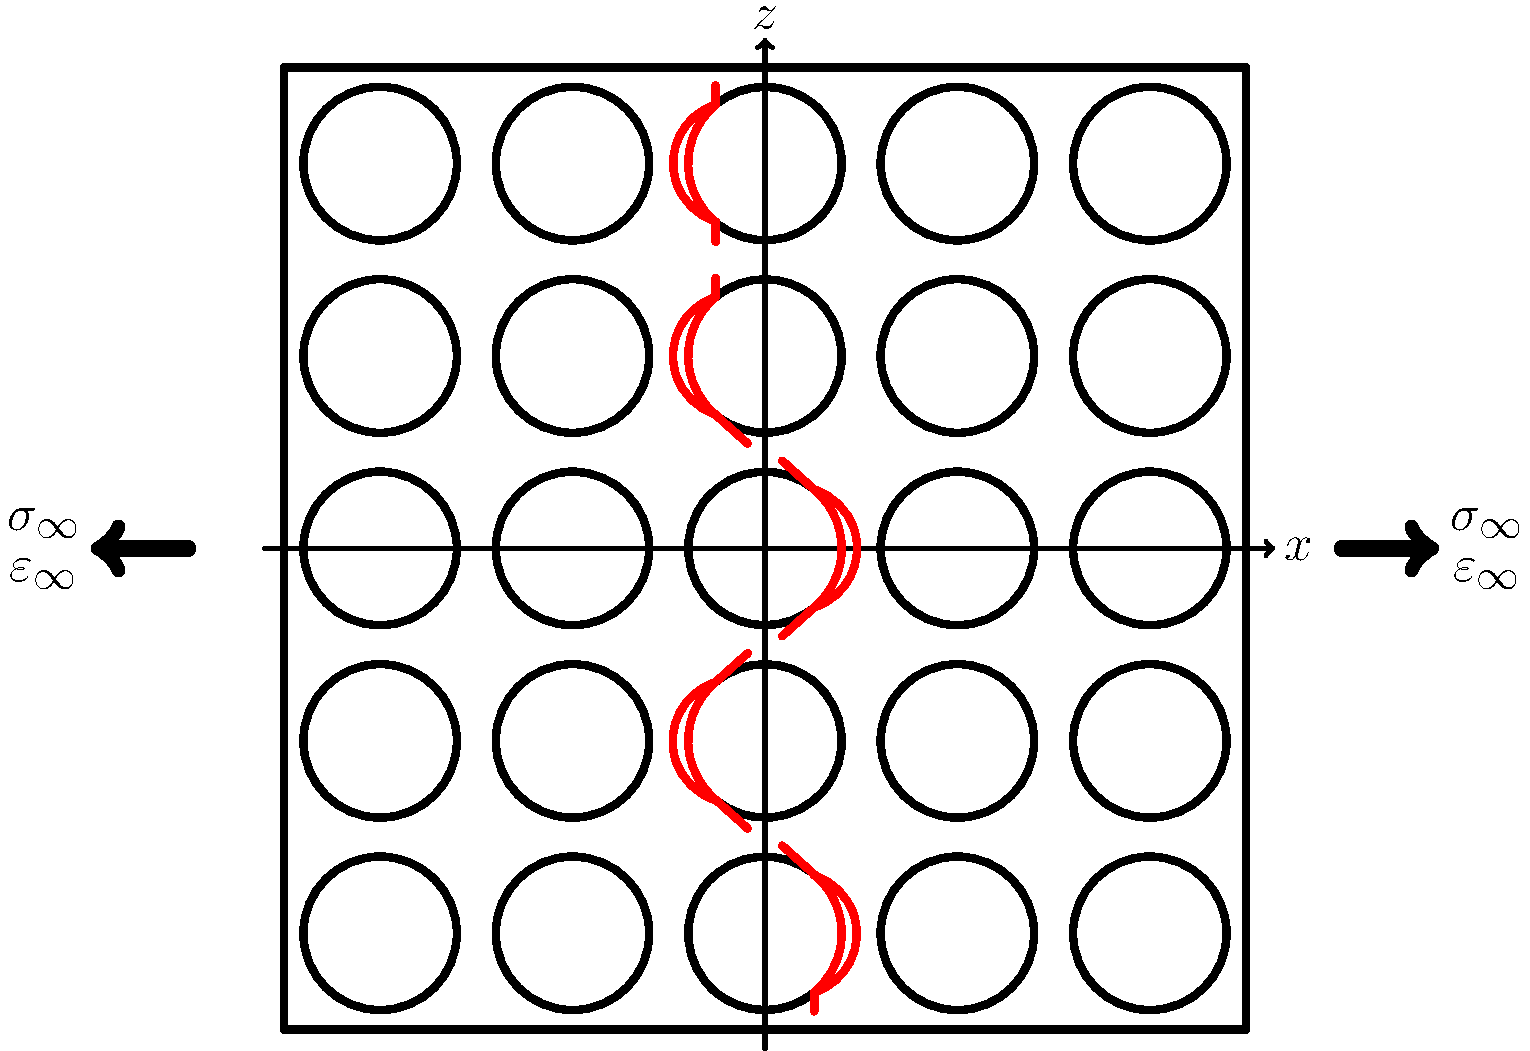
\includegraphics[width=\textwidth]{pics/stage3-kinking.pdf}
       \caption{Kinking.}\label{intro:fig:schematic-transversecracks-c}
    \end{subfigure}
    ~
    \begin{subfigure}[b]{0.45\textwidth}
        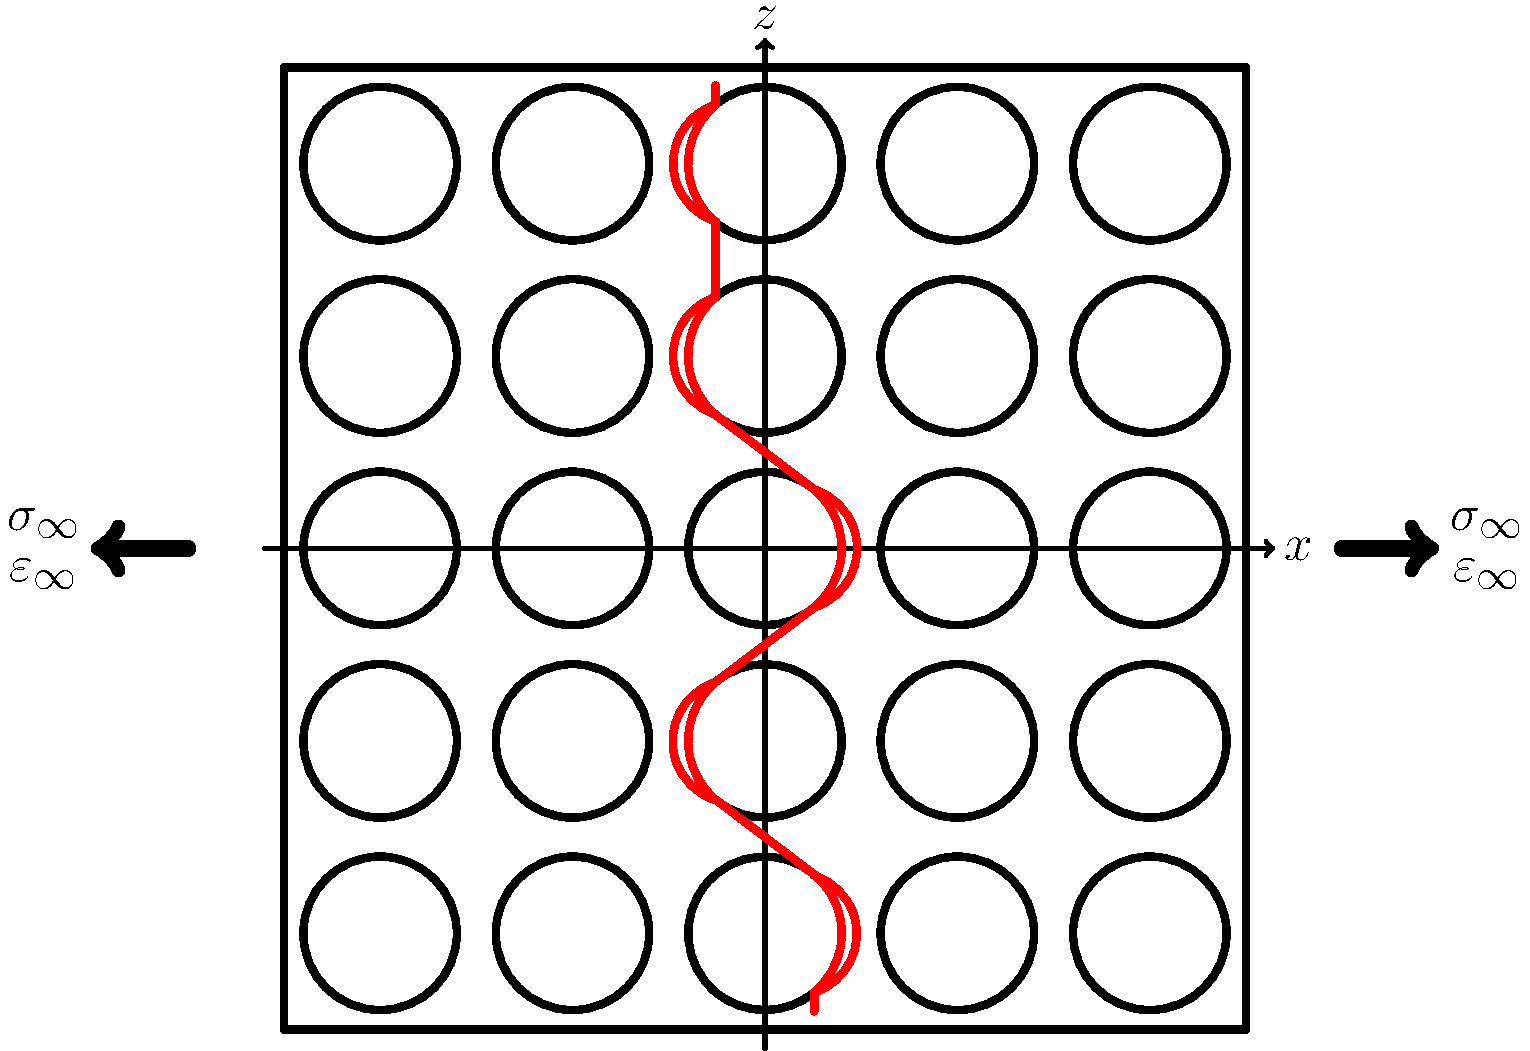
\includegraphics[width=\textwidth]{pics/stage4-coalescence.pdf}
       \caption{Coalescence.}\label{intro:fig:schematic-transversecracks-d}
    \end{subfigure}

\caption{Schematic representation of the formation of a transverse crack across the ply thickness.}\label{intro:fig:schematic-transversecracks}
\end{figure}

The description of the microscopic origin of transverse cracking presented previously leads naturally to the conclusion that a correct understanding of the \emph{ply-thickness effect} and of the mechanisms that delay and suppress transverse cracking in thin-ply laminates requires a thorough comprehension of fiber/matrix debonding.\\
Different approaches have been adopted to model the fiber/matrix interface crack and provide a theoretical understanding of debonding process. One of the most widely used method is the Cohesive Zone Model (CZM), which has been employed to simulate simultaneously the onset and propagation of debonds along multiple fiber interfaces~\cite{Kushch2011,Canal2012,Bouhala2013,Herraez2015}. Used in conjunction with a failure model for matrix, usually involving an elasto-plastic behavior with hardening~\cite{Canal2012,Herraez2015}, such modeling approach aims at computing the location of the transverse crack starting from a virgin, i.e. undamaged. material. It furthermore provides the global force-displacement response of the simulated specimen, which can be directly compared with the results from mechanical tests. Given the interest in reconstructing numerically the growth of a transverse crack, authors working with this approach have usually focused on large Representative Volume Elements (RVEs) with computer-generated pseudo-random fiber distributions~\cite{Intro:Segurado2002,Intro:Elnekhaily2018} or real fiber distributions reconstructed from microscopy imaging techniques. From the computational point of view, a Cohesive Zone Model coupled with an elasto-plastic matrix has the main advantage of avoiding any singularity in the stress and displacement fields at the crack tip, as it would occur in Linear Elastic Fracture Mechanics (LEFM) or Finite Fracture Mechanics (FFM). The crack tip itself is not directly modelled, on the other hand the fracture process is ``smeared'' over the finite length of the cohesive element~\cite{Bazant1983}. However, some drawbacks exists. First, a significant number of material properties are required as input of the model, most of which are not experimentally measurable at the microscopic level for fiber/matrix debonding. This leads to the adoption of properties measured at the macroscopic scale or the need to calibrate the numerical procedure with respect to specific macroscopic force-displacement responses~\cite{Canal2012}.The validity and applicability of such approach to then study an arbitrary configuration is an open question. Furthermore, the correct cancellation of the crack tip singularity, which is required to ensure accurate results, depends on Cohesive Elements length and it is thus sensitive to the mesh. For a bi-material interface crack as a debond under mixed-mode conditions, Jin and Sun~\cite{Jin2005} showed that a single cohesive zone length may not be able to cancel simultaneously both the tensile and shear stress singularity at the crack tip. They further observed that high values of the Cohesive Element tensile and shear stiffness are required to ensure a negligible energy dissipation at the cohesive zone tip.
Finally, the adoption of an elasto-plastic matrix in conjunction with the Cohesive Zone Model might not represent the actual physics of the failure process at the fiber/matrix interface. As mentioned before, the triaxiality of the matrix stress state in the inter-fiber region induces brittle failure of the matrix at or very close to the interface through a cavitation-like mechanism~\cite{Asp1995,Asp1996,Pawlak2014}. This process would create a small initial debond at the interface and then debond growth would occur starting from this initial flaw, a situation better modeled by the classic Griffith's criterion of Linear Elastic Fracture Mechanics (LEFM). In a LEFM analysis, Mode I and Mode II Energy Release Rate (ERR) at the crack tip are evaluated by means of the Virtual Crack Closure Technique (VCCT)~\cite{Krueger2004} and/or the J-Integral method~\cite{Rice1968}. Stress, strain and displacement fields are needed for the computation of the ERR and can be calculated using analytical solutions~\cite{Toya1974} as well as numerical methods, such as the Boundary Element Method (BEM)~\cite{Paris1996} or the Finite Element Method (FEM)~\cite{Zhuang2018}. Some limitations however exist. LEFM is in fact able to describe only propagation and not initiation of the debond. Furthermore, no agreement still exists among researchers on a propagation criteria that would correctly capture the mode-dependent behavior of the critical ERR at the interface. The interest in this thesis is to investigate debond growth and, by comparing the ERR in different configurations, understand which mechanism favors and which one prevents debond growth. Thus, Linear Elastic Fracture Mechanics is the approach adopted. Furthermore, in Paper E, initiation of debonds is analyzed using a simple approach compatible with the tenets of LEFM.

\section{The fiber-matrix interface crack in LEFM}

The problem of fiber/matrix debonding, called also the fiber/matrix interface crack problem, belongs to the category of bi-material interface cracks, i.e. cracks occurring at the interface between two dissimilar materials. This class of problems was first studied in the context of Linear Elastic Fracture Mechanics by Williams~\cite{Williams1959} in the 1950's. By using arguments of asymptotic analysis, he derived the stress distribution around an \emph{open} straight crack, i.e. a crack with faces nowhere in contact with each other for any size of the crack itself. He considered the crack as occurring between two infinite half-planes of dissimilar materials (the intended application of his work was in the field of earthquake engineering). He found the existence of a strong oscillatory behavior in the stress singularity at the crack tip of the form

\begin{equation}\label{intro:eq:singularitywilliams}
r^{-\frac{1}{2}}\sin\left(\varepsilon\log r\right)\quad\text{with}\quad\varepsilon=\frac{1}{2\pi}\log\left(\frac{1-\beta}{1+\beta}\right);
\end{equation}

in which $\beta$ is one of the two Dundurs~\cite{Dundurs1969} parameters used to characterize interfaces between dissimilar materials:

\begin{equation}\label{intro:eq:dundursbeta}
\beta=\frac{\mu_{2}\left(\kappa_{1}-1\right)-\mu_{1}\left(\kappa_{2}-1\right)}{\mu_{2}\left(\kappa_{1}+1\right)+\mu_{1}\left(\kappa_{2}+1\right)}
\end{equation}

where $\kappa=3-4\nu$ in plane strain and $\kappa=\frac{3-4\nu}{1+\nu}$ in plane stress, $\mu$ is the shear modulus, $\nu$ Poisson's coefficient, and indexes $1,2$ refer to the two bulk materials. Later, Erdogan~\cite{Erdogan1963} found that oscillatory region size is in the order of $10^{-6}a$, where $a$ is the size of the crack. Notice that the previous results depend on the mismatch in elastic properties at the interface and thus apply equally to the straight as well as to the circular bi-material interface crack (the fiber/matrix interface crack). Due the oscillatory nature of the stress singularity at the crack tip (Eq.~\ref{intro:eq:singularitywilliams}), Stress Intensity Factors (SIFs) are not correctly defined anymore, as the $\lim_{r\rightarrow 0}\sqrt{2\pi r}\sigma$ ceases to be finite and returns logarithmically infinite terms~\cite{Comninou1990}. Determination of Mode mixity at the crack tip is thus an ill-posed problem. For the same reason, evaluation of Mode I and Mode II Energy Release Rate at the debond tip is not possible. However, by evaluating the ERR over a finite length instead of an infinitesimal one, it is possible to compute an estimate of Mode I and Mode II ERR with reasonable accuracy. This leads naturally to the use of the Virtual Crack Closure Technique~\cite{Krueger2004}, which computes Mode I and Mode II ERR over a finite size.\\
In the \emph{open crack} case, the existence of an interpenetration zone close to the crack tip was found~\cite{England1965,Malyshev1965} with a length in the order of $10^{-4}$~\cite{England1965}. On the basis of considerations laid out in\cite{Malyshev1965}, Comninou~\cite{Comninou1977} introduced the presence of a \emph{contact zone} in the crack tip neighborhood, of a length to be determined from the solution of the elastic problem, showed that it provided a physically consistent solution to the problem of the straight bi-material interface crack.\\
England~\cite{England1966} and Perlman and Sih~\cite{Perlman1967} employed analytical tools to solve the fiber/matrix interface crack and computed the stress and displacement fields for a circular inclusion with respectively a single debond and an arbitrary number of debonds. Based upon their work, Toya~\cite{Toya1974} obtained the expression of the Energy Release Rate (ERR) of the \emph{open} debond.\\
The study of more complex configurations, rather than the single partially debonded fiber in an infinite matrix of~\cite{England1966,Perlman1967,Toya1974}, requires numerical treatment, thus numerical studies soon followed these first analytical solutions. Par{\'{\i}}s and colleagues~\cite{Paris1996} developed a Boundary Element Method (BEM) employing discontinuous singular elements at the crack tip and the Virtual Crack Closure Integral (VCCI)~\cite{Irwin1958} to compute the Energy Release Rate (ERR) at the debond tip. The method was initially developed for the \emph{open crack} case and was validated with respect to Toya's analytical results~\cite{Toya1974}. The effect of interface discretization on the accuracy of stress calculations in the debond tip neighborhood was later studied~\cite{DelCano1997}. Based on Comninou's work on the straight crack~\cite{Comninou1977}, the possibility of contact zone onset (\emph{closed crack} case) was considered to avoid interpenetration of debond faces~\cite{Paris1996}. The effect of the presence of a contact zone on debond ERR was analyzed in~\cite{Varna1997a}.

Their algorithm was then applied to investigate the fiber-matrix interface crack under different geometrical configurations and mechanical loadings ~\cite{Paris2007,Correa2007,Correa2011,Correa2013,Correa2014,Sandino2016,Sandino2018}.\\
Recently the Finite Element Method (FEM) was also applied to the solution of the fiber-matrix interface crack problem~\cite{Zhuang2018,Varna2017,Zhuang2018a}, in conjunction with the Virtual Crack Closure Technique (VCCT)~\cite{Rybicki1977,Krueger2004} for the evaluation of the ERR at the crack tip. In~\cite{Zhuang2018}, the authors validated their model with respect to the BEM results of~\cite{Paris1996}, but no analysis of the effect of the discretization in the crack tip neighborhood comparable to~\cite{DelCano1997} was proposed. Thanks to the interest in evaluating the ERR of interlaminar delamination, different studies exist in the literature on the effect of mesh discretization on Mode I and Mode II ERR of the bi-material interface crack when evaluated with the VCCT in the context of the FEM~\cite{Sun1987,Manoharan1990,Sun1997}.

The bimaterial interface crack problem belongs to the class of \emph{receding contact}~\cite{Paris1996,Garrido1991}, i.e. such that the contact zone in the final configuration is smaller than in the initial one. It was shown that this class of problems has some peculiar properties~\cite{Keer1972,Tsai1974}, which are valid both with and without friction at the interface~\cite{Paris1996,Garrido1991}: size and shape of the contact zone remain the same upon a change in the magnitude of the applied load; only a change in the disposition of the applied load causes a change in the size and shape of the contact zone; displacements, stresses and strains (and consequently, Energy Release Rate) are directly proportional to the value of the applied load.

\section{Objectives of the thesis}

The main objective of the thesis is to investigate the effect of the composite microstructure on debond growth, characterized by its Mode I and Mode II Energy Release Rate. The aim is to understand which mechanisms cause an increase in the ERR, and thus favor the growth of debonds, and which mechanisms lead to a reduction of the ERR at the debond tip, and thus have a mitigating effect on debond growth. Both Uni-Directional (UD) composites (Paper B, Paper D, Paper E) and cross-ply laminates (Paper C and Paper E) are studied, and the aspects of interest are:

\begin{itemize}
\item the fiber volume fraction (Paper B);
\item the interaction between debonds in the loading direction (Paper B and Paper C);
\item the interaction between debonds in the through-the-thickness direction (Paper D);
\item the presence of a free surface and its distance from the debond (Paper B);
\item the presence of the $0^{\circ}/90^{\circ}$ interface and its distance from the debond (Paper C);
\item the thickness of the layer in which debonding occurs (the UD composite in Paper B, the $90^{\circ}$ layer in Paper C);
\item the thickness of the $0^{\circ}$ layer in cross-ply laminates (Paper C).
\end{itemize}

A second aim is to estimate the initial size of debonds after initiation and the final maximum size of debonds after propagation and how these are affected by the microstructural feature previously highlighted (Paper E). Given the oscillatory behavior of the LEFM crack-tip solution of the fiber/matrix interface crack problem (see previous section), a further objective is to determine the convergence behavior of the Virtual Crack Closure Technique used in conjunction with the Finite Element Method to compute debond Energy Release Rate.
